%!TEX root = ../thesis.tex
% appendix section 7

\chapter{Electrical impedance measurement}
\label{sec:ap7}

This section will cover a side topic about the atmospheric pressure plasma generated by a microwave resonator and the electrical impedance measurement of such plasma. Atmospheric pressure plasma is all different from strongly coupled plasma, belonging to a region that a traditional plasma theory can explain (see Fig.\ref{fig:taxonomy}). It is a topic which is actively investigated both in theories and applications in a couple of decades thanks to its simple apparatus such as the absence of a vacuum chamber. Before diving into the subjects of strongly coupled plasma presented in this thesis, I spent about three years researching the atmospheric pressure plasma field and learning the fundamentals of plasma theory and experimental techniques, including various diagnostic methods. In particular, I improved a traditional method of measuring the impedance of the plasma generated by a microwave resonator and published journal papers \cite{lee2017situ, nam2017asymmetric}. A brief overview of the atmospheric pressure plasma, the microwave resonator, and the improved technique for measuring the plasma impedance will be introduced.

% -----
\section{Atmospheric pressure microwave plasma}
\label{sec:ap7-1}

Atmospheric pressure plasma, as the name implies, has the property of retaining its shape because the plasma pressure is equivalent to that of the atmosphere. As a result, no extra equipment for confining plasma, such as a chamber, is required, and the device may become a portable way. In particular, atmospheric pressure plasma generated using a microwave in the GHz band has a non-thermal feature that maintains a relatively low gas temperature compared to a high electron temperature \cite{tendero2006atmospheric}. In recent years, microwave discharges at atmospheric pressure are being explored for a wide range of applications, including biomedical \cite{lu2016reactive, graves2014low}, agriculture \cite{sera2008germination}, decontamination \cite{kuo2007fan}, and novel material synthesis \cite{kramer2015cold, vollath2008plasma}. 

In the various applied studies described above, measuring the electrical impedance of plasma is a vital subject in order to increase device efficiency, protect circuits, and calculate the coupled power purely to the plasma itself. Moreover, it is possible to diagnose plasma properties from the electrical impedance of the plasma. Therefore, the theoretical and experimental study on the implications of the electrical impedance of plasma and its measurement for various sources has been widely investigated \cite{lieberman2005principles, blackwell2005measurement, iza2005split, choi2009microwave, mckay2010excitation}.

The impedance of an electrical component $Z_\text{L}$ can be easily determined by measuring the reflection coefficient $\Gamma$ or  $S_\text{11}$ satisfying the relation
\begin{equation}
\Gamma \left( f \right) = \frac{Z_\text{L} \left( f \right) - Z_0}{Z_\text{L} \left( f \right) + Z_0}
\end{equation}
, where $Z_0$ is the characteristic impedance of the transmission line \cite{pozar2011microwave}. To make things simpler, the plasma impedance is calculated by measuring the reflection coefficient by regarding the plasma to be the load of a circuit. There is a problem that impedance consists of two parts -- real and imaginary values, but fortunately, since the above equation depends on the frequency, the impedance can be determined by measuring the reflection coefficient while changing the frequency $f$ of the microwave.

In general, it is not difficult to change the input frequency, and in some cases, it is possible to measure the reflection coefficient and scattering parameter (also known as S-parameter) according to the frequency at once using a network analyzer. However, in the case of plasma generated by a microwave resonator, since the energy transfer efficiency of the source itself is optimized at a specific frequency, it is impossible to change the frequency freely. The state of the plasma can be changed even within a narrow frequency range, and thus, there is a limitation in diagnosing the impedance of plasma in a non-destructive way \cite{iza2005split, choi2009microwave, park2010inactivation, kang2011slit, lee2015self}.

% -----
\section{Two-frequency diagnostics}
\label{sec:ap7-2}

\begin{figure}[h!]
\centering
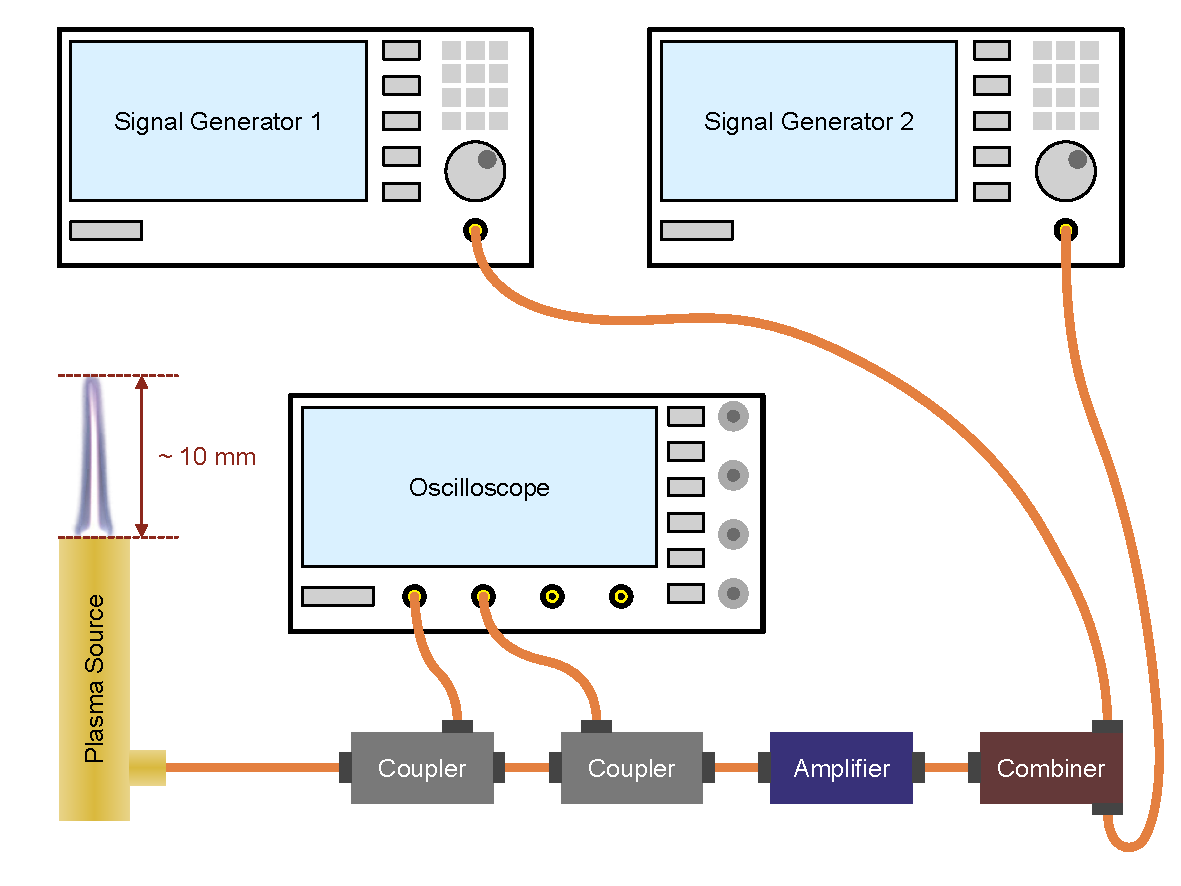
\includegraphics[width=100mm]{figures/ap7/twoFreq/twoFreq.pdf}
\caption{Schematic diagram of the two-frequency diagnostic method. Two different signal generators are implemented simultaneously for the main high power and the scanning low power signals together with the power combiner. The powers of the forward and reflected signals for the scanning frequency are measured with a couple of directional couplers and the oscilloscope.}
\label{fig:twoFreq}
\end{figure}

In order to circumvent the difficulties described above, we developed a method of measuring plasma impedance by using two signal generators, a power combiner, and directional couplers (Fig.\ref{fig:twoFreq}).  One of the signal generators produces the main microwave signal at a fixed frequency with high power, and the other generator varies the frequency of the output signal with low enough power for a scanning purpose that is not perturbing the plasma but still in a detectable level. The power combiner receives both the main and scanning signals, and the amplifier raises the signals. Two directional couplers take the forward and reflected signals in opposite directions connected in series.

This method allows the measurement of S11 over a relatively large frequency range and provides a more accurate determination of the plasma impedance than the conventional method. Moreover, this method makes it possible to measure the electrical impedance of plasma with high reliability and calculates the power coupled only to the plasma, excluding the amount of dissipation in the circuit and the device. 


